% Provenance (never printed): see sources/outline_sources.md (Year 1: solute and particle
% fluxes; the Hjulstrom diagram; settling velocity; denudation rates). Exercise and problem
% values in the Book 3 scratch calculator calc/ch20.py; figure data from
% figdata/bachelor-1/settling.py and threshold.py. Erosion, transport and deposition are
% Book 1's (g5); the sediment load in three forms, the denudation rate and isostatic rebound
% are Book 2's (g12), re-founded here (load, denudation rate) or recalled (rebound); discharge
% and the drainage basin are Book 2 g10's; Airy isostasy is ch. 11's; viscosity, Stokes' law
% and the Reynolds number are the physics books' (admitted, pointer). Grain-size classes and
% sorting belong to ch. 21.
\chapter{Erosie en transport}\label{ch:b1:erosion-transport}

Na een storm loopt de rivier onder de brug bruin. Het water dat de dag ervoor helder was, zit vol modder, draait om de pijlers en voert takken mee, en op de bedding, onzichtbaar, stoten kiezels tegen elkaar terwijl zij rollen. Elke seconde neemt de vloed tonnen land mee. Stroomafwaarts, achter een dam, bezinkt dezelfde modder in het stille water van het stuwmeer, dat elk jaar een beetje van zijn volume verliest; nog verder, bij de monding van de rivier, spreidt zij zich in de zee uit als een bruine pluim die vanuit de ruimte te zien is. Dit hoofdstuk geeft cijfers aan die reis: hoeveel een rivier meevoert en in welke vormen, hoe snel een korrel zinkt, welke stroming nodig is om haar in beweging te zetten, en hoe snel uiteindelijk een heel landschap wordt weggesleten.

\begin{recall}
Erosie is het afslijten van het land en het wegvoeren van de stukken; afzetting is het neerleggen ervan waar de drager vertraagt (Boek~1, klas~5). Een rivier voert haar sedimentvracht als \omterm{def:b1:erosion-transport:load}{bodemvracht}, \omterm{def:b1:erosion-transport:load}{zwevende vracht} en \omterm{def:b1:erosion-transport:load}{opgeloste vracht}; de erosiesnelheid van een regio is de dikte van gesteente die er per tijdseenheid van wordt weggehaald, in meter per miljoen jaar; wanneer erosie een dikte $e$ van de \omterm{def:b1:layered-earth:layers}{korst} wegneemt, zakt het oppervlak door isostatische terugveer slechts met $e(1 - \rho_c/\rho_m)$ (Boek~2, klas~12). De afvoer van een rivier is het volume water dat per tijdseenheid een doorsnede passeert, en haar stroomgebied het gebied dat haar voedt (Boek~2, klas~10). In \omterm{prop:b1:isostasy-gravity:airy}{Airy-isostasie} drijft de \omterm{def:b1:layered-earth:layers}{korst} op de \omterm{def:b1:layered-earth:layers}{mantel} met een wortel evenredig aan haar reliëf (\cref{prop:b1:isostasy-gravity:airy}). De \omterm{def:b1:weathering-clays:hydrolysis}{hydrolyse} van silicaten stuurt ionen en opgelost silica naar de rivieren (\cref{def:b1:weathering-clays:hydrolysis}). De dynamische viscositeit $\mu$ van een vloeistof meet haar weerstand tegen afschuiving, en de kinematische viscositeit is $\nu = \mu/\rho$; een bol met diameter $d$ die langzaam met snelheid $w$ door een vloeistof beweegt, ondervindt de weerstand $3\pi\mu d w$ (wet van Stokes); het Reynoldsgetal $w d/\nu$ vergelijkt de traagheid met de viskeuze krachten, en de stroming rond de bol is glad zolang hij klein blijft (de natuurkundeboeken).
\end{recall}

\section{Opgeloste en deeltjesfluxen}\label{sec:b1:erosion-transport:fluxes}

Een rivier verwijdert het land op twee manieren: als materie in oplossing, de producten van \omterm{def:b1:weathering-clays:weathering}{chemische verwering}, en als vaste korrels, de producten van \omterm{def:b1:weathering-clays:weathering}{fysische verwering} en de onoplosbare residuen van \omterm{def:b1:weathering-clays:weathering}{chemische verwering}. De twee reizen op verschillende manieren, en de korrels zelf reizen op twee manieren.

\begin{definition}[Opgeloste vracht, zwevende vracht, bodemvracht]\label{def:b1:erosion-transport:load}
De vracht van een rivier is de materie die zij langs een doorsnede meevoert, in drie delen die verschillen naar hoe zij reizen. De \emph{opgeloste vracht}\index{opgeloste vracht} is de materie in oplossing, ionen en opgelost silica, die met het water meebeweegt in zijn eigen snelheid. De \emph{zwevende vracht}\index{zwevende vracht} bestaat uit korrels die binnen de stroming door haar turbulentie worden opgehouden, vooral klei, silt en fijn zand, die bijna met de snelheid van het water bewegen en zelden de bodem raken. De \emph{bodemvracht}\index{bodemvracht} bestaat uit korrels die over de bodem rollen, glijden of springen, in voortdurend contact ermee, veel langzamer dan het water.
\end{definition}

\begin{omfigure}
\begin{tikzpicture}[font=\footnotesize, >={Stealth[length=4pt]}]
% schematic: the three loads of a river (side view) and the forces on a bed grain
\fill[omDef!12] (0,0) rectangle (9,3.2);
\draw[omDef!80!black, thick] (0,3.2) -- (9,3.2);
\node[anchor=south west, omDef!80!black] at (0,3.2) {wateroppervlak};
% flow profile arrows (velocity grows upward)
\foreach \y/\l in {0.35/0.5, 0.8/0.9, 1.4/1.15, 2.1/1.3, 2.8/1.4} {\draw[->, black!55] (0.25,\y) -- ++(\l,0);}
\draw[black!55] (0.25,0.12) -- (0.25,3.05);
\node[anchor=north west, black!65, align=left] at (0.2,-0.15) {stroomsnelheid\\ profiel};
% bed
\fill[black!12] (0,-0.05) rectangle (9,0.12);
\foreach \x in {0.1,0.45,...,8.9} {\fill[black!45] (\x,0.0) circle[radius=0.09];}
% dissolved load: ions
\foreach \x/\y/\s in {2.3/2.7/+, 3.1/1.9/-, 4.0/2.85/+, 4.7/2.2/-, 5.6/2.75/+, 6.3/1.85/+, 7.2/2.6/-, 8.2/2.2/+, 2.7/1.2/-, 7.8/1.3/-} {\node[circle, draw=omThm, inner sep=0.2pt, minimum size=7pt, font=\tiny, text=omThm] at (\x,\y) {$\s$};}
% suspended load: fine grains, denser near the bed
\foreach \x/\y in {2.1/1.5, 2.6/0.9, 3.0/2.5, 3.4/0.6, 3.7/1.4, 4.2/0.8, 4.4/1.9, 4.9/0.55, 5.2/1.2, 5.5/2.1, 5.9/0.7, 6.1/1.5, 6.6/0.9, 6.9/2.3, 7.4/0.6, 7.6/1.7, 8.0/0.85, 8.5/1.4, 3.9/0.45, 5.0/0.35, 6.4/0.4, 2.4/0.45, 8.6/0.5} {\fill[brown!75!black] (\x,\y) circle[radius=0.05];}
% bed load: rolling and hopping grains
\fill[black!60] (3.2,0.27) circle[radius=0.15];
\draw[->, black!70] (3.0,0.55) arc[start angle=150, end angle=30, radius=0.25];
\fill[black!60] (5.6,0.25) circle[radius=0.12];
\draw[->, black!70, densely dashed] (4.6,0.2) .. controls (4.9,0.9) and (5.3,0.7) .. (5.55,0.4);
\fill[black!60] (4.6,0.22) circle[radius=0.06];
% labels
\node[omThm, anchor=west] at (9.2,2.5) {opgeloste vracht: ionen};
\node[brown!75!black, anchor=west] at (9.2,1.5) {zwevende vracht:};
\node[brown!75!black, anchor=west] at (9.2,1.1) {klei, silt, fijn zand};
\node[black!75, anchor=west] at (9.2,0.4) {bodemvracht: rollend,};
\node[black!75, anchor=west] at (9.2,0.0) {glijdende, springende korrels};
\draw[->, thick, black!70] (6.8,3.55) -- node[above] {stroming} (8.6,3.55);
% inset: forces on a grain resting on two others; it pivots about its downstream contact
\begin{scope}[xshift=11.8cm, yshift=-2.2cm]
  \fill[black!12] (-1.2,-0.4) rectangle (1.2,0);
  \fill[black!40] (-0.6,-0.15) circle[radius=0.28]; \fill[black!40] (0.6,-0.15) circle[radius=0.28];
  \fill[black!65] (0,0.166) circle[radius=0.4];
  \draw[->, thick, omDef!80!black] (0,0.166) -- (0,1.15) node[above] {lift};
  \draw[->, thick, omThm] (0,0.166) -- (1.05,0.166) node[right] {weerstand};
  \draw[->, thick, black] (0,0.166) -- (0,-0.8) node[below] {gewicht in water};
  \draw[->, thick, black!60] (-1.4,0.85) -- (-0.5,0.85) node[pos=0, left] {stroming};
  \fill[red!60!black] (0.353,-0.020) circle[radius=0.045];
  \node[font=\scriptsize, anchor=north west, black!70] at (0.5,-0.4) {draaipunt};
\end{scope}
\end{tikzpicture}

{\small De drie vrachten van een rivier, van opzij gezien (schematisch, niet op schaal). De stroming is het snelst nabij het oppervlak en wordt nul op de bodem. Ionen zijn over de hele diepte verspreid; zwevende korrels worden door de wervels meegevoerd, meer ervan nabij de bodem; bodemvrachtkorrels rollen, glijden of maken korte sprongen. Rechts: de krachten op een korrel van de bodem. De weerstand en de lift van de stroming proberen haar over haar benedenstroomse buur te rollen, om het contactpunt; haar gewicht in het water houdt haar tegen.}
\label{fig:b1:erosion-transport:loads}
\end{omfigure}

De grens tussen de twee vaste vrachten wordt niet door de korrelgrootte vastgelegd: zij hangt van de stroming af. Een vloed die zand in zwevende toestand meevoert, laat het bij het wegebben op de bodem achter, als \omterm{def:b1:erosion-transport:load}{bodemvracht}; de fijnste klei daarentegen blijft in bijna elke stroming in zwevende toestand en wordt nauwelijks op de bodem van een stromende rivier gevonden. Elke vracht wordt gemeten als een flux, een massa per tijdseenheid door een doorsnede van de rivier.

\begin{proposition}[Flux van een vracht]\label{prop:b1:erosion-transport:flux}
Laat $c$ de concentratie van een opgeloste of \omterm{def:b1:erosion-transport:load}{zwevende vracht} zijn (massa per volume-eenheid water) en $u$ de snelheid van het water, beide variërend over de doorsnede met oppervlak $A$. (1)~De momentane flux van de vracht door de doorsnede is
\[
  F = \iint_A c\,u\,\mathrm dA = \overline{c}_Q\,Q,
\]
waarbij $Q = \iint_A u\,\mathrm dA$ de afvoer is en $\overline{c}_Q$ de gemiddelde concentratie gewogen met de snelheid. (2)~Over een periode $T$ waarin de afvoer $Q(t)$ en de concentratie $C(t)$ van de rivier variëren, is de meegevoerde massa
\[
  M = \int_0^T Q\,C\,\mathrm dt = T\left(\overline{Q}\;\overline{C} +
  \operatorname{cov}(Q, C)\right),
\]
waarbij de streepen tijdgemiddelden zijn en $\operatorname{cov}(Q, C)$ het gemiddelde van $(Q - \overline{Q})(C - \overline{C})$ is. Het product van de gemiddelde afvoer en de gemiddelde concentratie geeft de juiste massa alleen als beide ongecorreleerd zijn.
\end{proposition}

\begin{proof}
(1)~In een tijd $\mathrm dt$ vult het water dat een klein oppervlak $\mathrm dA$ van de doorsnede kruist een volume $u\,\mathrm dA\,\mathrm dt$, dat de massa $c\,u\,\mathrm dA\,\mathrm dt$ meevoert; het optellen over de doorsnede geeft $F$, en $\overline{c}_Q$ wordt gedefinieerd als $F/Q$. (2)~Schrijf $Q = \overline{Q} + Q'$ en $C =
\overline{C} + C'$, waarbij de fluctuaties $Q'$ en $C'$ over de periode gemiddeld nul zijn. Dan is $QC = \overline{Q}\,\overline{C} + \overline{Q}\,C' + Q'\,\overline{C}
+ Q'C'$; de twee middelste termen middelen tot nul, en het gemiddelde van $Q'C'$ is de covariantie.
\end{proof}

De covariantie is van belang voor de \omterm{def:b1:erosion-transport:load}{zwevende vracht}. Haar concentratie stijgt sterk bij vloeden, wanneer de regen grond in de beken spoelt en de snellere stroming korrels van de bodem opheft, zodat $Q$ en $C$ samen toenemen: een groot deel van de jaarlijkse sedimentvracht van een rivier passeert in een paar dagen van vloed, en een meetcampagne die hen mist, of een gemiddelde concentratie vermenigvuldigd met de gemiddelde afvoer, onderschat de vracht. De \omterm{def:b1:erosion-transport:load}{opgeloste vracht} gedraagt zich andersom: vloeden verdunnen haar, en haar concentratie is het hoogst bij lage afvoer, wanneer de rivier wordt gevoed door grondwater dat lang in contact is geweest met het gesteente.

\begin{method}[De jaarlijkse vracht van een rivier uit meting]\label{met:b1:erosion-transport:gauging}
\begin{enumerate}
  \item Registreer de afvoer continu bij een meetstation.
  \item Bemonster het water bij veel afvoeren, ook die van vloeden, en meet de massa sediment per liter (door filtreren en wegen) en van elke opgeloste soort.
  \item Weeg de concentraties met de afvoer op het moment van bemonstering, om de door de stroming gewogen gemiddelde concentratie te krijgen, of fit de concentratie als functie van de afvoer en pas die toe op de hele reeks.
  \item Vermenigvuldig met het totale volume water van het jaar, of tel $Q\,C\,\Delta
        t$ op over de reeks (\cref{prop:b1:erosion-transport:flux}).
  \item Voeg de \omterm{def:b1:erosion-transport:load}{bodemvracht} toe, die watermonsters missen, uit aparte metingen of als geschatte fractie.
  \item Verwijder voor de \omterm{def:b1:erosion-transport:load}{opgeloste vracht} wat niet uit het gesteente komt: de zouten die door regen worden aangevoerd en, voor het bicarbonaat, de koolstof die uit de lucht is opgenomen (\cref{ch:b1:weathering-clays}).
\end{enumerate}
\end{method}

\begin{omfigure}
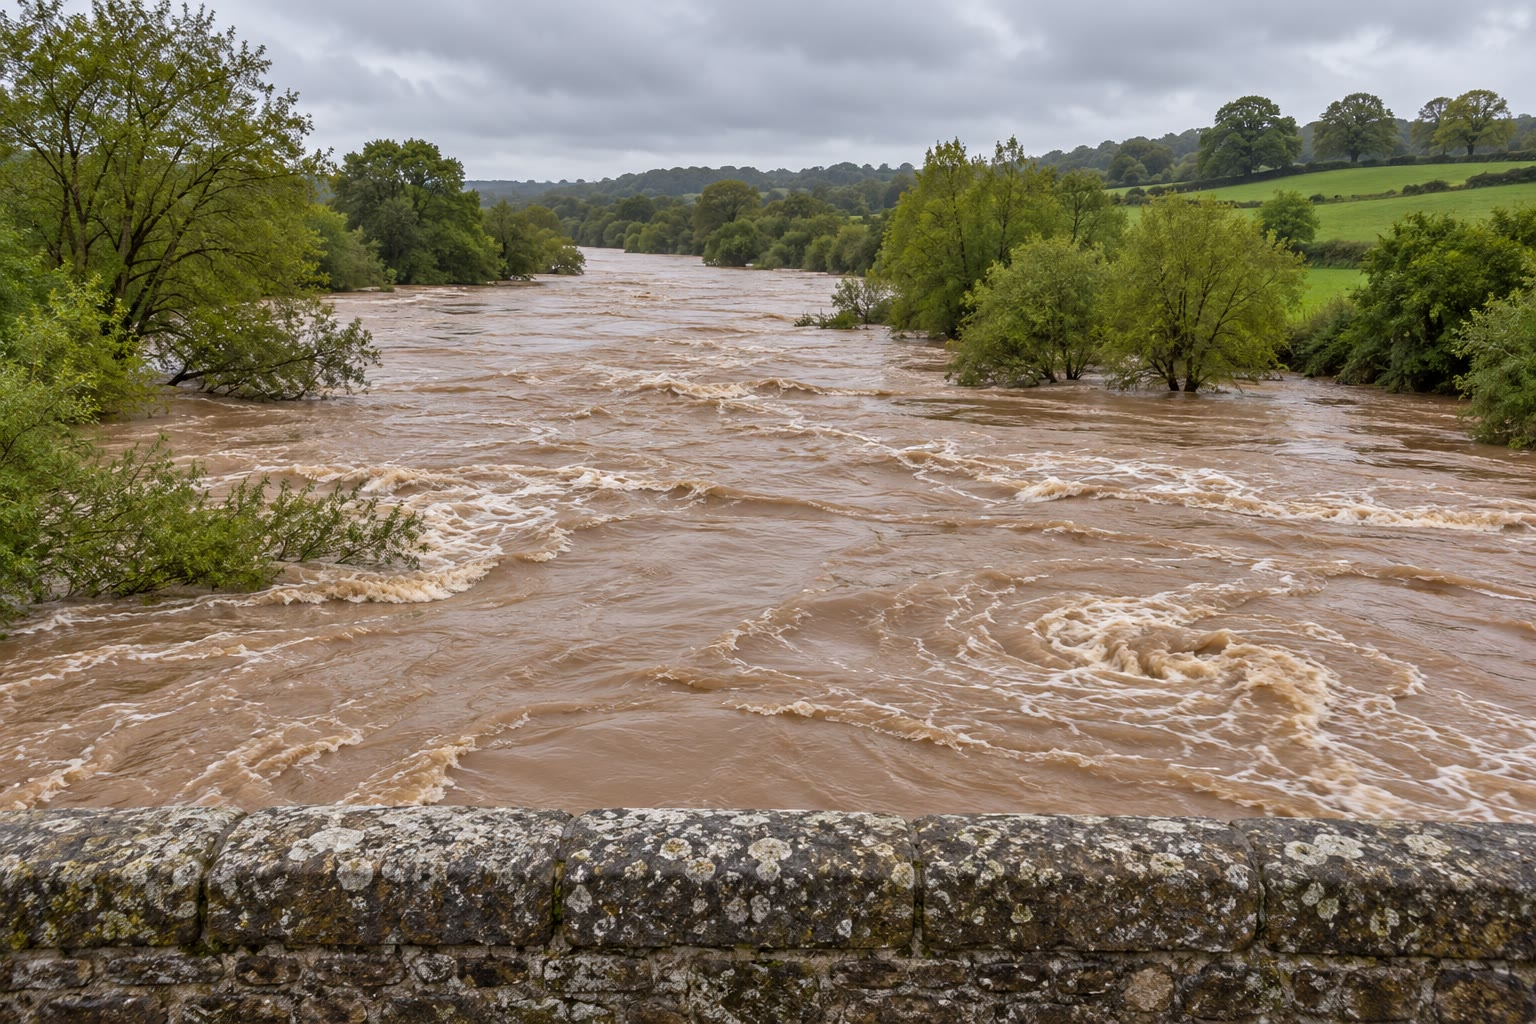
\includegraphics[height=5.1cm]{images/book3/ai/b1-muddy-river.jpg}\hfill
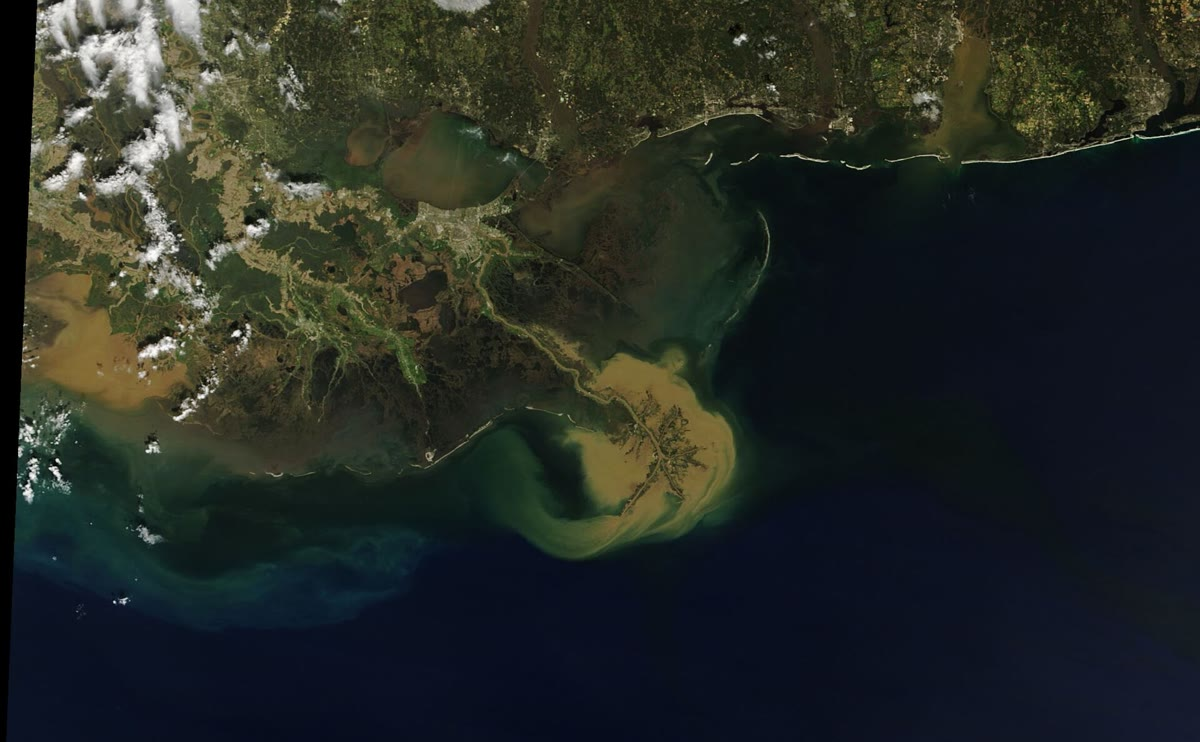
\includegraphics[height=5.1cm]{images/book3/b1-mississippi-plume.jpg}
\par\smallskip{\small Links: een rivier in vloed voert bruin, met sediment beladen water (AI-illustratie). Rechts: de vloedpluim van de Mississippi die in de Golf van Mexico uitstroomt rond zijn delta, gezien door het MODIS-instrument op de satelliet Terra op 4~maart 2018; de zwevende modder kleurt de zee bruin en groen, en de zuidoostenwind duwt de pluim naar het noordwesten. NASA Earth Observatory-beeld door Joshua Stevens, publiek domein, via Wikimedia Commons.}
\label{fig:b1:erosion-transport:plume}
\end{omfigure}
% ledger: commons:mississippi-plume

\emph{De wereldrivieren.} Vóór enige menselijke invloed voerden de rivieren van de wereld naar schatting \qty{14}{Gt} zwevend sediment per jaar naar de kustoceaan, \qty{15.5}{Gt} met de \omterm{def:b1:erosion-transport:load}{bodemvracht}. De mens heeft beide uiteinden van de reis veranderd: landbouw en ontbossing hebben de bodemerosie verhoogd, en voegen ongeveer \qty{2.3}{Gt} per jaar aan de rivieren toe, terwijl stuwmeren sediment tegenhouden: de grote houden ongeveer \qty{20}{\percent} van de flux vast en de kleine nog eens \qty{6}{\percent}, en meer dan \qty{100}{Gt} sediment ligt nu achter dammen, vooral gebouwd in de afgelopen vijftig jaar. Het netto effect is een vermindering: de moderne flux is ongeveer \qty{12.6}{Gt} per jaar.
% ledger: syvitski:flux

\begin{dated}{2005}
De cijfers voor de flux van zwevend sediment, vóór en na menselijke invloed, komen uit een wereldmodel van rivierensediment dat in 2005 is gepubliceerd. Sindsdien zijn er dammen bijgebouwd.
\end{dated}
% ledger: syvitski:flux

Het opgeloste deel is kleiner. Een klassieke compilatie van riviermetingen, in 1963 gemaakt, zette de opgeloste materie die de rivieren van de wereld naar de zee brengen op ongeveer \qty{3.9}{Gt} per jaar, ongeveer \qty{30}{\percent} van de moderne zwevende flux, bij een gemiddelde concentratie van \qty{120}{mg} per liter. Bicarbonaat maakt bijna de helft ervan uit, \qty{58}{mg.L^{-1}}, gevolgd door calcium, silica, sulfaat, chloride en natrium. Een deel ervan komt niet uit het gesteente: veel van het bicarbonaat draagt koolstof die uit de lucht of de bodem is opgenomen, en een deel van het chloride en het natrium komt van zeezout dat door de regen wordt meegevoerd. Afzonderlijke rivieren wijken sterk van deze gemiddelden af.
% ledger: livingstone:world-dissolved, syvitski:flux

\emph{Het sedimentbudget van een bekken.} Niet elke korrel die in een stroomgebied wordt geërodeerd, bereikt de uitlaat. Van een veld weggespoelde grond kan aan de voet van de helling blijven liggen, zand kan eeuwenlang in de uiterwaarde en in de zandbanken van de rivier worden opgeslagen, en een stuwmeer kan het grootste deel van wat erin komt tegenhouden. De vracht die aan de uitlaat wordt gemeten, is het saldo van het budget: wat op de hellingen en uit de oevers wordt geërodeerd, minus wat onderweg wordt opgeslagen, plus wat uit oude voorraden wordt teruggenomen. Over een paar decennia meten kan dit saldo ver van de langetermijnsnelheid van erosie liggen, in beide richtingen, wat een van de redenen is voor de andere methoden van \cref{sec:b1:erosion-transport:denudation}.

\section{Bezinksnelheid}\label{sec:b1:erosion-transport:settling}

Een korrel is dichter dan water en zinkt. Of een rivier haar kan meevoeren, en waar zij zal worden afgezet, hangt in de eerste plaats af van hoe snel zij zinkt.

\begin{definition}[Bezinksnelheid]\label{def:b1:erosion-transport:settling}
De \emph{bezinksnelheid}\index{bezinksnelheid} $w_s$ van een korrel is de constante snelheid waarmee zij door stilstaand water valt, wanneer de weerstand van het water haar onderwaterse gewicht in evenwicht houdt, haar gewicht minus de opwaartse kracht van het water dat zij verplaatst.
\end{definition}

Een korrel die in stilstaand water wordt losgelaten, versnelt tot haar weerstand, die met haar snelheid groeit, haar onderwaterse gewicht in evenwicht houdt; voor een zand- of siltkorrel kost dit een kleine fractie van een seconde, zodat de \omterm{def:b1:erosion-transport:settling}{bezinksnelheid} de snelheid is waarmee zij bijna de hele weg valt. Met de dichtheden $\rho_s$ van de korrel en $\rho$ van het water schrijven we $R = (\rho_s - \rho)/\rho$ voor de relatieve onderwaterse dichtheid.

\begin{proposition}[Stokes-bezinking]\label{prop:b1:erosion-transport:stokes}
Een bol met diameter $d$ en dichtheid $\rho_s$ die langzaam door water met dichtheid $\rho$ en dynamische viscositeit $\mu$ valt, volgens de wet van Stokes, heeft de \omterm{def:b1:erosion-transport:settling}{bezinksnelheid}
\[
  w_s = \frac{(\rho_s - \rho)\,g\,d^2}{18\,\mu} = \frac{R\,g\,d^2}{18\,\nu}.
\]
De wet geldt zolang het korrel-Reynoldsgetal $w_s d/\nu$ onder ongeveer 1 blijft, dat wil zeggen voor diameters beneden $d_1 = \left(18\,\nu^2/(R\,g)\right)^{1/3}$.
\end{proposition}

\begin{proof}
De weging van de bol is $\rho_s g\,\pi d^3/6$ en de opwaartse kracht $\rho g\,\pi d^3/6$, dus is zijn onderwaterse gewicht $(\rho_s - \rho)\,g\,\pi d^3/6$. Bij de \omterm{def:b1:erosion-transport:settling}{bezinksnelheid} is het gelijk aan de weerstand $3\pi\mu d\,w_s$:
\[
  (\rho_s - \rho)\,g\,\frac{\pi d^3}{6} = 3\pi\mu d\,w_s
  \quad\Longrightarrow\quad
  w_s = \frac{(\rho_s - \rho)\,g\,d^2}{18\,\mu},
\]
en het delen van teller en noemer door $\rho$ geeft de tweede vorm.
Het Reynoldsgetal van deze snelheid is $R g d^3/(18\nu^2)$, dat gelijk is aan 1 voor $d = d_1$ en groeit als $d^3$.
\end{proof}

Voor kwarts, met dichtheid \qty{2650}{kg.m^{-3}}, in water van \qty{20}{\celsius}, met dichtheid \qty{998.2}{kg.m^{-3}} en viscositeit \qty{1.0016}{mPa.s}: $R =
1.65$, $\nu = \qty{1.003e-6}{m^2.s^{-1}}$, en met $g =
\qty{9.81}{m.s^{-2}}$ is de grens $d_1 = \qty{0.104}{mm}$, een fijn zand. Daaronder geeft de wet van Stokes de bezinksnelheden van silt en klei: een siltkorrel van \qty{10}{\micro m} over sinkt met \qty{9.0e-5}{m.s^{-1}}, \qty{1}{m} in ongeveer drie uur; een kleideeltje van \qty{2}{\micro m} met \qty{3.6e-6}{m.s^{-1}}, \qty{1}{m} in \num{3.2}~dagen. Natuurlijke kleideeltjes zijn schilfers, geen bollen, en zinken nog langzamer. Water van \qty{5}{m} diep, volkomen stil, zou zestien dagen nodig hebben om van zulke klei te worden ontdaan; een stromende rivier, waarvan de wervels het steeds weer opwerpen, doet dat nooit, en daarom reist het fijnste slib naar zee.
% ledger: hom:quartz, nist:water, const:gn

Boven $d_1$ groeit de weerstand sneller dan evenredig met de snelheid: het water dat langs de korrel stroomt, scheidt zich erachter in een zog, en bij grote Reynoldsgetallen is de weerstand evenredig met het kwadraat van de snelheid. Experimenten op natuurlijke korrels zijn samengevat in één formule die de twee regimes verbindt.

\begin{proposition}[Gecombineerde bezinkingswet]\label{prop:b1:erosion-transport:combined}
De \omterm{def:b1:erosion-transport:settling}{bezinksnelheid} van natuurlijke korrels met zeefdiameter $d$ is, voor alle groottes,
\[
  w_s = \frac{R\,g\,d^2}{C_1\,\nu + \sqrt{0.75\,C_2\,R\,g\,d^3}},
\]
met $C_1 = 18$ en $C_2 = 1.0$.
\end{proposition}
\admitted
% ledger: fc:settling

De wet is van Ferguson en Church, die haar fitten op gemeten bezinksnelheden van natuurlijke zanden. Voor kleine korrels is de vierkantswortel verwaarloosbaar en reduceert zij tot de wet van Stokes; voor grote korrels is de eerste term van de noemer verwaarloosbaar en $w_s \to \sqrt{4 R g d/(3 C_2)}$, dat alleen als de vierkantswortel van de grootte groeit. De constanten hangen van de vorm van de korrels af: $C_2 = 0.4$ beschrijft gladde bollen, grotere waarden hoekiger korrels, die meer weerstand ondervinden. De twee wetten gaan boven \qty{0.1}{mm} uiteen. Voor een korrel van \qty{1}{mm} geeft de gecombineerde wet \qty{0.126}{m.s^{-1}}, zeven keer minder dan de wet van Stokes; voor een kiezel van \qty{10}{mm}, \qty{0.46}{m.s^{-1}} tegenover een zinloze \qty{90}{m.s^{-1}} (diagram hieronder).
% ledger: fc:settling

\begin{omfigure}
\begin{tikzpicture}[font=\small]
% settling velocity of quartz grains in water at 20 C (figdata/bachelor-1/settling.py)
\begin{axis}[width=11cm, xmode=log, ymode=log, xmin=0.001, xmax=10, ymin=1e-8, ymax=10, height=8cm,
    xlabel={korreldiameter $d$ (\si{mm})}, ylabel={bezinksnelheid (\si{m.s^{-1}})},
    ytick={1e-8,1e-6,1e-4,1e-2,1},
    legend style={at={(0.03,0.97)}, anchor=north west, font=\footnotesize}, legend cell align=left,
    grid=major, grid style={black!10}]
  \addplot[omDef, thick, dashed] table[x=d_mm, y=w_stokes] {figdata/out/bachelor-1-settling-curves.dat};
  \addplot[omThm, very thick] table[x=d_mm, y=w_fc] {figdata/out/bachelor-1-settling-curves.dat};
  \legend{wet van Stokes, gecombineerde wet (natuurlijke korrels)}
  \draw[black!55, densely dotted] (axis cs:0.1037,1e-7) -- (axis cs:0.1037,10);
  \node[font=\scriptsize, anchor=west, align=left, black!75] at (axis cs:0.115,1e-6) {korrel-Reynoldsgetal\\  $= 1$};
  \node[font=\scriptsize, black!70] at (axis cs:0.002,3e-8) {klei};
  \node[font=\scriptsize, black!70] at (axis cs:0.016,3e-8) {silt};
  \node[font=\scriptsize, black!70] at (axis cs:0.35,3e-8) {zand};
  \node[font=\scriptsize, black!70] at (axis cs:4.5,3e-8) {grind};
  \draw[black!40] (axis cs:0.0039,1e-8) -- (axis cs:0.0039,1e-7);
  \draw[black!40] (axis cs:0.0625,1e-8) -- (axis cs:0.0625,1e-7);
  \draw[black!40] (axis cs:2,1e-8) -- (axis cs:2,1e-7);
\end{axis}
\end{tikzpicture}

{\small \omterm{def:b1:erosion-transport:settling}{Bezinksnelheid} van kwartskorrels in water van \qty{20}{\celsius} tegen hun diameter, beide op logaritmische schalen: de wet van Stokes en de gecombineerde wet van natuurlijke korrels, berekend. Op deze schalen is de wet van Stokes een rechte lijn met helling 2. De twee komen overeen voor silt en klei; boven ongeveer \qty{0.1}{mm}, waar het korrel-Reynoldsgetal 1 overschrijdt, vertraagt de weerstand van het zog de grove korrels. De streepjes onderaan markeren de grenzen van de korrelgrootteklassen, bij \qty{3.9}{\micro m} ($1/256$~mm), \qty{62.5}{\micro m} ($1/16$~mm) en \qty{2}{mm}.}
\label{fig:b1:erosion-transport:settling}
\end{omfigure}
% ledger: fc:settling, usgs:wentworth-phi

Over het bereik van het diagram, van de fijnste klei tot grof grind, bestrijkt de \omterm{def:b1:erosion-transport:settling}{bezinksnelheid} acht ordes van grootte. Dit is de eerste reden waarom rivieren hun sediment sorteren: een afnemende stroming laat haar grind meteen vallen, haar zand binnen meters, haar silt binnen kilometers, en voert haar klei naar een meer of naar zee. De korrelgroottenklassen en de sortering van sedimenten zijn het onderwerp van het volgende hoofdstuk (\cref{ch:b1:clastic-sediments}).

\section{Beginbeweging en het diagram van Hjulström}\label{sec:b1:erosion-transport:threshold}

Een korrel die in rust op de bodem van een rivier ligt, wordt in beweging gezet door de kracht van het water dat erover stroomt. Die kracht wordt gemeten door een spanning.

\begin{definition}[Bodemschuifspanning, schuifsnelheid]\label{def:b1:erosion-transport:bed-shear}
De \emph{bodemschuifspanning}\index{bodemschuifspanning} $\tau_b$ van een stroming is de kracht per oppervlakte-eenheid die zij op haar bodem uitoefent, evenwijdig aan de bodem, in de richting van de stroming. De schuifsnelheid is $u_* = \sqrt{\tau_b/\rho}$, een snelheid die dezelfde spanning meet.
\end{definition}

De \omterm{def:b1:erosion-transport:bed-shear}{bodemschuifspanning} kan niet worden afgelezen van een stroommeter, maar in een stationaire stroming volgt zij uit een krachtenevenwicht.

\begin{proposition}[Diepte-helling-product]\label{prop:b1:erosion-transport:depth-slope}
In een stationaire, uniforme stroming met diepte $h$ door een brede geul met kleine helling $S$ is de \omterm{def:b1:erosion-transport:bed-shear}{bodemschuifspanning}
\[
  \tau_b = \rho\,g\,h\,S .
\]
\end{proposition}

\begin{proof}
Beschouw het water boven een stuk bodem van lengte $L$ langs de stroming en van eenheidsbreedte, waarbij de geul zo breed is dat de oevers kunnen worden genegeerd. De stroming is stationair en uniform, dus versnelt dit water niet en houden de krachten erop elkaar in evenwicht. De drukkrachten op zijn stroomopwaartse en stroomafwaartse vlakken zijn gelijk en tegengesteld, omdat de diepte op beide gelijk is. Langs de stroming blijven over de component van het gewicht, $\rho g h L \sin\beta$, waarbij $\beta$ de hoek van de bodem is, en de wrijving van de bodem, $\tau_b L$, ertegenin. Dus $\tau_b
= \rho g h \sin\beta$, en voor een kleine hoek is $\sin\beta \approx \tan\beta = S$.
\end{proof}

Een rivier van \qty{2}{m} diep op een helling van \num{0.001}, een meter val per kilometer, heeft $\tau_b = 998.2 \times 9.81 \times 2 \times 0.001 =
\qty{19.6}{Pa}$, en een schuifsnelheid van \qty{0.140}{m.s^{-1}}. In een geul die niet breed is, nemen de oevers hun deel van de wrijving voor hun rekening, en wordt de diepte vervangen door de hydraulische straal, de oppervlakte van de doorsnede gedeeld door haar natte omtrek (\cref{exo:b1:erosion-transport:5}).

\emph{Krachten op een korrel.} De stroming duwt een korrel van de bodem met haar weerstand en tilt haar op door de snellere stroming over haar top (de inzet van de eerste figuur van dit hoofdstuk). Beide krachten werken op het oppervlak van de korrel, dus schalen zij als $\tau_b
d^2$; de korrel weerstaat met haar onderwaterse gewicht, dat schaalt als $(\rho_s - \rho) g d^3$. De verhouding van de twee is de natuurlijke maat voor de sterkte van de stroming voor een gegeven korrel.

\begin{definition}[Shields-parameter, drempel van beweging]\label{def:b1:erosion-transport:threshold}
De \emph{Shields-parameter}\index{Shields-parameter} van een stroming met \omterm{def:b1:erosion-transport:bed-shear}{bodemschuifspanning} $\tau_b$ over korrels met diameter $d$ en dichtheid $\rho_s$ is
\[
  \theta = \frac{\tau_b}{(\rho_s - \rho)\,g\,d}.
\]
De \emph{drempel van beweging}\index{drempel van beweging} van de korrels is de \omterm{def:b1:erosion-transport:bed-shear}{bodemschuifspanning}, of de waarde $\theta_c$ van de Shields-parameter, waarbij zij beginnen te bewegen.
\end{definition}
% ledger: hecras:thresholds

De kritische waarde $\theta_c$ wordt in goten gemeten, en de metingen vallen op één kromme wanneer zij worden uitgezet tegen een dimensieloze korrelgrootte die de korrel en de vloeistof combineert.

\begin{proposition}[Drempelkromme van Soulsby en Whitehouse]\label{prop:b1:erosion-transport:soulsby}
Voor korrels met diameter $d$ op een vlakke bodem, met
$D_* = d\,\left(R\,g/\nu^2\right)^{1/3}$, is de kritische \omterm{def:b1:erosion-transport:threshold}{Shields-parameter}
\[
  \theta_c = \frac{0.3}{1 + 1.2\,D_*} + 0.055\left(1 - e^{-0.02\,D_*}\right),
\]
en de kritische \omterm{def:b1:erosion-transport:bed-shear}{bodemschuifspanning} is $\tau_c = \theta_c\,(\rho_s - \rho)\,g\,d$.
\end{proposition}
\admitted
% ledger: hecras:thresholds

Voor grove korrels nadert $\theta_c$ \num{0.055}: grind beweegt wanneer de \omterm{def:b1:erosion-transport:bed-shear}{bodemschuifspanning} ongeveer een twintigste bereikt van het onderwaterse gewicht van een laag korrels van één diameter dik, per oppervlakte-eenheid. Sedimenttransportformules die een constante drempel gebruiken, nemen waarden van \num{0.03} tot \num{0.047}, het laatste in de klassieke bodemvrachtformule van Meyer-Peter en Müller. Voor fijn zand stijgt $\theta_c$ weer, tot \num{0.077} bij \qty{0.1}{mm}: kleine korrels liggen in de trage, viskeuze laag water dicht bij de bodem en worden door hun buren beschermd. Het minimum, \num{0.030}, ligt bij ongeveer \qty{0.7}{mm}. In pascal groeit de drempel altijd met de grootte (diagram hieronder): \qty{0.13}{Pa} voor een zand van \qty{0.1}{mm}, \qty{0.51}{Pa} bij \qty{1}{mm}, \qty{9.0}{Pa} bij \qty{10}{mm}, \qty{57}{Pa} voor een kei van \qty{64}{mm}.
% ledger: hecras:thresholds

\begin{omfigure}
\begin{tikzpicture}[font=\small]
% threshold of motion of quartz grains in water at 20 C (figdata/bachelor-1/threshold.py, Soulsby and Whitehouse)
\begin{axis}[name=a, width=6.9cm, height=6cm, xmode=log, xmin=0.0625, xmax=100, ymin=0, ymax=0.12,
    xlabel={korreldiameter $d$ (\si{mm})}, ylabel={kritische Shields-parameter $\theta_c$},
    yticklabel style={/pgf/number format/fixed, /pgf/number format/precision=2},
    grid=major, grid style={black!10}, title={\footnotesize (a) dimensieloos}]
  \addplot[omThm, very thick] table[x=d_mm, y=theta] {figdata/out/bachelor-1-threshold-shields.dat};
  \draw[black!50, dashed] (axis cs:0.0625,0.055) -- (axis cs:100,0.055) node[pos=0.7, above, font=\scriptsize, black!70] {$0.055$};
\end{axis}
\begin{axis}[at={(a.east)}, anchor=west, xshift=2.0cm, width=6.9cm, height=6cm, xmode=log, ymode=log,
    xmin=0.0625, xmax=100, ymin=0.05, ymax=200,
    xlabel={korreldiameter $d$ (\si{mm})}, ylabel={kritische bodemschuifspanning $\tau_c$ (\si{Pa})},
    grid=major, grid style={black!10}, title={\footnotesize (b) in pascal}]
  \addplot[omDef, very thick] table[x=d_mm, y=tau_cr] {figdata/out/bachelor-1-threshold-shields.dat};
\end{axis}
\end{tikzpicture}

{\small De \omterm{def:b1:erosion-transport:threshold}{drempel van beweging} van kwartskorrels in water van \qty{20}{\celsius}, uit de kromme van Soulsby en Whitehouse, berekend van de grens van fijn zand (\qty{0.0625}{mm}) tot de grootte van een kei. (a)~De kritische \omterm{def:b1:erosion-transport:threshold}{Shields-parameter} is bijna constant voor grind en stijgt voor fijn zand. (b)~De kritische \omterm{def:b1:erosion-transport:bed-shear}{bodemschuifspanning} groeit bijna evenredig met de diameter voor grind.}
\label{fig:b1:erosion-transport:threshold}
\end{omfigure}
% ledger: hecras:thresholds

\begin{example}[Wat de rivier verplaatst]\label{ex:b1:erosion-transport:river}
In de rivier van \qty{2}{m} diep op een helling van \num{0.001}, $\tau_b =
\qty{19.6}{Pa}$. Voor korrels van \qty{20}{mm} is $\theta = 19.6/(1651.8 \times
9.81 \times 0.020) = 0.060$, net boven hun drempel van \num{0.055}: zij bewegen. Voor korrels van
\qty{40}{mm} is $\theta = 0.030$, de helft van de drempel: zij blijven liggen. De rivier verplaatst
haar bodem tot grof grind; voor zand van \qty{1}{mm} is
$\theta = 1.21$, bijna veertig keer de drempel van \num{0.031}.
\end{example}

\emph{In suspensie.} Eenmaal in beweging hopt een korrel langs de bodem of wordt zij in de stroming opgenomen, afhankelijk van de vraag of de wervels, waarvan de snelheden van de orde van de schuifsnelheid zijn, haar tegen haar bezinking kunnen ophouden.

\begin{proposition}[Criterium van suspensie]\label{prop:b1:erosion-transport:suspension}
Een korrel met \omterm{def:b1:erosion-transport:settling}{bezinksnelheid} $w_s$ kan alleen in een turbulente stroming in suspensie blijven als sommige wervels sneller omhoog gaan dan zij zinkt. Omdat de opwaartse snelheden van de wervels van de orde van de schuifsnelheid $u_*$ zijn, begint suspensie wanneer $u_*$ $w_s$ nadert en is zij volledig ontwikkeld wanneer $u_*$ hem overschrijdt; dit hoofdstuk neemt $u_* = w_s$ als de grens van suspensie.
\end{proposition}
\admitted
% ledger: bagnold:suspension

In de rivier van het voorbeeld is $u_* = \qty{0.140}{m.s^{-1}}$, wat de gecombineerde bezinkingswet geeft aan korrels van \qty{1.16}{mm}: zand dat fijner is dan ongeveer een millimeter reist in suspensie, grover zand en grind als \omterm{def:b1:erosion-transport:load}{bodemvracht}. Het argument gaat terug op Bagnold, die opmerkte dat korrels van \qty{0.1}{mm} of minder volledig in suspensie zijn zodra zij bewegen, terwijl korrels groter dan \qty{1}{mm} een \omterm{def:b1:erosion-transport:bed-shear}{bodemschuifspanning} nodig hebben die vele keren hun drempel is. Wanneer de vloed wegebt en $u_*$ daalt, valt het grove zand als eerste terug op de bodem.

\emph{Van spanning tot gemiddelde snelheid.} Wat in een rivier makkelijk wordt gemeten of geschat, is haar gemiddelde snelheid. In een turbulente stroming over een bodem die door korrels met diameter $d$ is opgeruwd, heeft een brede geul met diepte $h$ de gemiddelde snelheid $U = u_*\left(6.25 + 5.75\log_{10}(h/d)\right)$, een wet die Keulegan in 1938 vaststelde uit de experimenten van Nikuradse en Bazin, zodat de \omterm{def:b1:erosion-transport:threshold}{drempel van beweging} overeenkomt met de kritische gemiddelde snelheid
\[
  U_c = \left(6.25 + 5.75\,\log_{10}\frac{h}{d}\right)\sqrt{\theta_c\,R\,g\,d},
\]
en de grens van suspensie, $u_* = w_s$, naar $U_s = \left(6.25 +
5.75\log_{10}(h/d)\right) w_s$. Beide hangen van de diepte af, maar alleen via een logaritme.
% ledger: keulegan:mean-velocity, bagnold:suspension

Drempelsnelheden horen dus bij één diepte en één reeks wetten: berekend voor een andere diepte, of afgelezen uit andere metingen, komen zij anders uit. Uitgezet tegen de korrelgrootte is hun vorm robuust maar hun waarden niet, en de \omterm{def:b1:erosion-transport:bed-shear}{bodemschuifspanning}, die niet op dezelfde manier van de diepte afhangt, is de betere maat van wat een stroming kan. De snelheden zijn nog steeds intuïtiever, en de klassieke manier om ze weer te geven is een diagram.

\begin{definition}[Diagram van Hjulström]\label{def:b1:erosion-transport:hjulstrom}
Een \emph{diagram van Hjulström}\index{diagram van Hjulström} zet de gemiddelde snelheid van een stroming uit tegen de diameter van de korrels, op logaritmische schalen, en verdeelt het vlak in de velden waarin korrels in rust worden geërodeerd, korrels die al bewegen in transport blijven, en bewegende korrels worden afgezet.
\end{definition}
% ledger: hjulstrom:curve

\begin{omfigure}
\begin{tikzpicture}[font=\small]
% Hjulstrom-type diagram for a flow 1 m deep (figdata/bachelor-1/threshold.py); the hatched
% cohesive field is schematic (its lower edge, 30 cm/s, is not computed)
\begin{axis}[width=12cm, height=8.4cm, xmode=log, ymode=log, xmin=0.001, xmax=100, ymin=0.1, ymax=3000,
    xlabel={korreldiameter $d$ (\si{mm})}, ylabel={gemiddelde stroomsnelheid (\si{cm.s^{-1}})},
    unbounded coords=jump, grid=major, grid style={black!10}]
  \addplot[draw=none, name path=dep] table[x=d_mm, y=u_dep] {figdata/out/bachelor-1-threshold-hjul.dat};
  \addplot[draw=none, name path=bot] coordinates {(0.001,0.1) (100,0.1)};
  \addplot[fill=omDef!14, draw=none] fill between[of=dep and bot];
  \fill[pattern=north east lines, pattern color=omThm!45] (axis cs:0.001,30) rectangle (axis cs:0.0625,3000);
  \addplot[omThm, very thick] table[x=d_mm, y=u_cr] {figdata/out/bachelor-1-threshold-hjul.dat};
  \addplot[omDef, very thick, dashed] table[x=d_mm, y=u_s] {figdata/out/bachelor-1-threshold-hjul.dat};
  \node[font=\footnotesize, fill=white, fill opacity=0.85, text opacity=1, align=center] at (axis cs:0.5,1500) {\textbf{erosie}: korrels die in suspensie worden meegevoerd};
  \node[font=\footnotesize, fill=white, fill opacity=0.85, text opacity=1, align=center] at (axis cs:22,330) {\textbf{bodemvracht}};
  \node[font=\footnotesize, fill=white, fill opacity=0.85, text opacity=1, align=center] at (axis cs:0.0042,2.5) {\textbf{transport}:\\ reeds bewegende\\ korrels blijven\\ in suspensie};
  \node[font=\footnotesize, fill=white, fill opacity=0.85, text opacity=1, align=center] at (axis cs:3,0.6) {\textbf{afzetting}};
  \node[font=\footnotesize, fill=white, fill opacity=0.85, text opacity=1, align=center] at (axis cs:0.008,300) {cohesieve modder:\\ drempel bepaald door\\ compactie};
  \node[font=\scriptsize, omThm, anchor=north, rotate=12] at (axis cs:6,80) {drempel van beweging};
  \node[font=\scriptsize, omDef, anchor=north west, rotate=57] at (axis cs:0.028,0.95) {grens van suspensie};
  \draw (rel axis cs:0,0) -- (rel axis cs:1,0);
\end{axis}
\end{tikzpicture}

{\small Een diagram van het type Hjulström voor kwartskorrels in water van \qty{1}{m} diep bij \qty{20}{\celsius}, berekend: de \omterm{def:b1:erosion-transport:threshold}{drempel van beweging} (doorgetrokken) uit de kromme van Soulsby en Whitehouse, de grens van suspensie (gestreept) uit de gecombineerde bezinkingswet, beide omgezet in gemiddelde snelheden met de wet van Keulegan. Boven de doorgetrokken kromme worden korrels in rust geërodeerd; onder de laagste van de twee krommen (gearceerd) worden bewegende korrels afgezet. Korrels fijner dan \qty{0.13}{mm} gaan in suspensie zodra zij bewegen; grovere reizen eerst als \omterm{def:b1:erosion-transport:load}{bodemvracht}. De berekening geldt alleen voor losse korrels: het gearceerde veld van cohesief silt en klei is schematisch.}
\label{fig:b1:erosion-transport:hjulstrom}
\end{omfigure}
% ledger: hecras:thresholds, fc:settling, bagnold:suspension, keulegan:mean-velocity

\emph{Het diagram lezen.} Drie kenmerken dragen de geologie. Ten eerste zijn de makkelijkste korrels om te eroderen fijne zanden, tussen ongeveer \num{0.06} en \qty{0.2}{mm}, die een stroom van \qtyrange{31}{34}{cm.s^{-1}} in beweging zet in water van \qty{1}{m} diep; grovere korrels hebben meer nodig, tot ongeveer \qty{3}{m.s^{-1}} voor een kei van \qty{64}{mm}. Ten tweede zijn silt en klei, hoewel zij lichter zijn, moeilijker te eroderen dan fijn zand zodra zij zijn bezonken: hun deeltjes kleven aan elkaar, en een gecompacteerde modder weerstaat een stroom die zand zou wegvegen. De berekening voor losse korrels kan dit niet zien, en de gemeten erosiesnelheden van modder variëren met hun compactie en watergehalte, vandaar het gearceerde veld. Ten derde gaat de kloof tussen erosie en afzetting voor de fijne korrels wijd open: een kleideeltje heeft een sterke stroom nodig om van een modderige bodem te worden losgerukt, maar eenmaal in het water blijft het in de zachtste stroming, en dat is de hele geschiedenis van de bruine vloed en van de pluim in zee.
% ledger: hjulstrom:curve, hecras:thresholds, keulegan:mean-velocity

\begin{history}[Twee studies uit de jaren dertig]
In 1935 publiceerde Filip Hjulström van het Geografisch Instituut van Uppsala een lange studie van het werk van de rivier de Fyris, in centraal Zweden, die het diagram bevatte dat zijn naam draagt: erosie- en afzettingssnelheden tegen de korrelgrootte, op logaritmische schalen. Anders dan eerdere krommen had zijn erosiekromme een minimum, tussen ongeveer \num{0.1} en \qty{0.5}{mm}: los fijn zand is het makkelijkst te eroderen, terwijl grover zand en grind, en ook silt en klei, die samenkleven, sterkere stromingen nodig hebben. Een jaar later, in 1936, de ingenieur A.~Shields,
in het proefschrift dat hij aan de Technische Hochschule van Berlijn verdedigde, zette de \omterm{def:b1:erosion-transport:threshold}{drempel van beweging} uit als een verhouding van krachten, de parameter die nu zijn naam draagt, tegen een dimensieloze korrelgrootte. De snelheden van Hjulström negeren de diepte van de stroming; de dimensieloze benadering van Shields doet dat niet, en zij ligt aan de basis van de drempelformules die vandaag worden gebruikt, zoals die achter de diagrammen van dit hoofdstuk.
\end{history}
% ledger: hjulstrom:curve, shields:1936, hecras:thresholds

\section{Afslijtingssnelheden}\label{sec:b1:erosion-transport:denudation}

De vrachten van een rivier, opgeteld over haar stroomgebied, meten hoe snel het stroomgebied wordt afgesleten.

\begin{definition}[Afslijtingssnelheid]\label{def:b1:erosion-transport:denudation}
De \emph{afslijtingssnelheid}\index{afslijtingssnelheid} $D$ van een regio is de gemiddelde snelheid waarmee het verwijderen van materie, als vaste korrels en in oplossing, haar oppervlak verlaagt, uitgedrukt als de equivalente dikte van vers gesteente per tijdseenheid, in meter per miljoen jaar (\unit{m/Myr}, hetzelfde als millimeter per duizend jaar). De massa die per oppervlakte-eenheid en tijdseenheid wordt weggehaald, in ton per vierkante kilometer per jaar, is de specifieke sedimentopbrengst.
\end{definition}

\begin{proposition}[Afslijting uit de vrachten van rivieren]\label{prop:b1:erosion-transport:denudation}
Als een stroomgebied met oppervlak $A$ via zijn uitlaat de jaarlijkse massa's $F_s$ van \omterm{def:b1:erosion-transport:load}{zwevende vracht}, $F_b$ van \omterm{def:b1:erosion-transport:load}{bodemvracht} en $F_d$ van \omterm{def:b1:erosion-transport:load}{opgeloste vracht} verliest die uit zijn gesteenten komen, en als er onderweg niets wordt opgeslagen, is zijn \omterm{def:b1:erosion-transport:denudation}{afslijtingssnelheid}
\[
  D = \frac{F_s + F_b + F_d}{\rho_r\,A},
\]
met $\rho_r$ de dichtheid van het verse gesteente. Voor $\rho_r =
\qty{2700}{kg.m^{-3}}$ komt een specifieke opbrengst van \qty{100}{t.km^{-2}.yr^{-1}} overeen met \qty{37}{m/Myr}.
\end{proposition}

\begin{proof}
De massa die per oppervlakte-eenheid en tijdseenheid verloren gaat, is $(F_s + F_b + F_d)/A$; gedeeld door de dichtheid van het gesteente wordt zij de dikte van gesteente die per tijdseenheid verloren gaat. Voor de omrekening is \qty{100}{t.km^{-2}.yr^{-1}} gelijk aan
$\qty{1e5}{kg}/\qty{1e6}{m^2} = \qty{0.1}{kg.m^{-2}}$ per jaar, of
$0.1/2700 = \qty{3.7e-5}{m}$ per jaar, \qty{37}{m} per miljoen jaar.
\end{proof}

De \omterm{def:b1:erosion-transport:load}{opgeloste vracht} telt alleen voor het deel dat uit het gesteente komt, niet uit de lucht: de koolstof van het bicarbonaat van silicaatverwering wordt uit de atmosfeer genomen, en alleen de kationen en het silica zijn gesteente. Het chemische deel van de afslijting is niet klein. Waar het klimaat warm en nat is en het reliëf laag, kan het het mechanische deel naderen of overtreffen, terwijl in steile bergen het mechanische deel overheerst.

\emph{Drie klokken.} De \omterm{def:b1:erosion-transport:denudation}{afslijtingssnelheid} kan over drie zeer verschillende tijdsruimten worden gemeten. Rivierenvrachten integreren jaren tot decennia, en zijn overgeleverd aan de paar vloeden die wel of niet plaatsvonden tijdens de metingen. Het sediment dat in een stuwmeer of een meer wordt gevangen, gemeten door de bodem ervan op te meten, integreert de decennia tot een eeuw van zijn bestaan. De derde klok staat geschreven in de korrels zelf, door kosmische straling.

\begin{proposition}[Kosmogene nucliden en erosie]\label{prop:b1:erosion-transport:cosmogenic}
Stel dat een nuclide in een gesteente door kosmische straling wordt geproduceerd met de snelheid $P(z) = P_0\,e^{-\rho z/\Lambda}$ per massa-eenheid, exponentieel afnemend met de diepte $z$ ($\rho$ de dichtheid van het gesteente, $\Lambda$ een constante, de verzwakkingslengte uitgedrukt als een massa per oppervlakte-eenheid), en dat het oppervlak met de constante snelheid $\varepsilon$ wordt verlaagd. Met verwaarlozing van radioactief verval draagt een korrel die het oppervlak bereikt de concentratie
\[
  N = \frac{P_0\,\Lambda}{\rho\,\varepsilon}.
\]
\end{proposition}

\begin{proof}
Ten opzichte van het oppervlak, dat met snelheid $\varepsilon$ zakt, stijgt een korrel met snelheid $\varepsilon$, dus brengt zij de tijd $\mathrm dz/\varepsilon$ door in een laag van dikte $\mathrm dz$ op diepte $z$, en verkrijgt zij daar de concentratie $P(z)\,\mathrm dz/\varepsilon$. Van grote diepte opkomend, bereikt zij het oppervlak met
\[
  N = \frac{1}{\varepsilon}\int_0^{\infty} P_0\,e^{-\rho z/\Lambda}\,\mathrm dz
  = \frac{P_0}{\varepsilon}\,\frac{\Lambda}{\rho}. \qedhere
\]
\end{proof}

De concentratie is omgekeerd evenredig met de erosiesnelheid: een langzaam eroderend oppervlak houdt elke korrel lang dicht bij het oppervlak en laadt haar met nucliden. De snelheid die het geeft, is gemiddeld over de tijd die nodig is om de paar meters te eroderen waarin de productie is geconcentreerd, dat wil zeggen van ongeveer duizend tot een miljoen jaar, afhankelijk van de snelheid. Het verwaarlozen van het verval is gerechtvaardigd wanneer die tijd kort is ten opzichte van de levensduur van het nuclide; wanneer de erosie zeer traag is, wordt het verval meegenomen en wordt de formule iets langer.
% ledger: portenga:method

\begin{inthelab}[Beryllium-10 in rivierzand]
Het gebruikelijke nuclide is beryllium-10, anders uitzonderlijk zeldzaam aan het oppervlak van de Aarde, dat door kosmische straling in het kwarts van de bovenste paar meter gesteente wordt gemaakt. Om de \omterm{def:b1:erosion-transport:denudation}{afslijtingssnelheid} van een heel bekken te meten, verzamelen geochemici zand uit de bedding van de rivier nabij de uitlaat, in de veronderstelling dat de rivier korrels van elke helling van het bekken mengt in verhouding tot de snelheid waarmee elk wordt geërodeerd. In het laboratorium wordt het kwarts van de andere mineralen gescheiden en gereinigd met zuren die het beryllium verwijderen dat in de lucht is gemaakt en door de regen is neergebracht; het wordt dan opgelost, een bekende hoeveelheid gewoon beryllium wordt toegevoegd, en het beryllium wordt geëxtraheerd. Zijn isotopen worden één atoom tegelijk geteld met een versneller-massaspectrometer, die de zeldzame beryllium-10-atomen kan vinden tussen een enorme overmaat van het gewone isotoop.
\end{inthelab}
% ledger: portenga:method

\emph{Wat de snelheden zijn.} Een compilatie van \num{1599} zulke metingen, in 2011 gepubliceerd, vond dat kale rotsbanken langzaam worden verlaagd: met \qty{12}{m/Myr} gemiddeld, met een mediaan van \qty{5.4}{m/Myr} (450 \omterm{def:b1:geological-maps:geological-map}{ontsluitingen}). Sedimentair gesteente slijt sneller weg, \qty{20}{m/Myr} gemiddeld, dan metamorf gesteente, \qty{11}{m/Myr}, en stollingsgesteente, \qty{8.7}{m/Myr}. Hele stroomgebieden verliezen veel meer, \qty{218}{m/Myr} gemiddeld met een mediaan van \qty{54}{m/Myr} (\num{1149} bekkens): hun steile hellingen, aardverschuivingen en rivierbeddingen eroderen veel sneller dan hun kale toppen, en een paar zeer snelle bekkens verhogen het gemiddelde vier keer boven de mediaan. De gemiddelde helling van een bekken is de beste enkelvoudige voorspeller van zijn snelheid. Bekkens in seismisch actieve regio's, waar bergen rijzen, geven gemiddeld \qty{367}{m/Myr}, tegenover \qty{182}{m/Myr} in rustige regio's; poolbekkens, door gletsjers uitgeschuurd, \qty{537}{m/Myr}; droge bekkens \qty{100}{m/Myr}.
% ledger: portenga:rates

\emph{\omterm{def:b1:isostasy-gravity:isostasy}{Isostasie} vertraagt het verlagen.} Het verwijderen van gesteente uit een regio in \omterm{def:b1:isostasy-gravity:isostasy}{isostasie} maakt haar kolommen lichter, en de \omterm{def:b1:layered-earth:layers}{korst} stijgt om het evenwicht te herstellen. Met $\rho_c
= \qty{2700}{kg.m^{-3}}$ en $\rho_m = \qty{3300}{kg.m^{-3}}$ (\cref{ch:b1:isostasy-gravity}), geeft de terugveerformule die aan het begin van het hoofdstuk werd herinnerd een verlaging van slechts $1 - 2700/3300 = 0.18$ van de verwijderde dikte: om het gemiddelde oppervlak van een regio met \qty{1}{m} te verlagen, moet de erosie \qty{5.5}{m} gesteente verwijderen. De tijd om een bergketen af te slijten is dus meer dan vijf keer wat haar hoogte gedeeld door haar \omterm{def:b1:erosion-transport:denudation}{afslijtingssnelheid} suggereert, en de gesteenten die nu aan het oppervlak liggen van oude, afgesleten ketens lagen eens vele kilometers diep. En omdat de terugveer de gemiddelde verwijderde dikte volgt, niet de verdeling ervan, stijgt een keten waarvan de dalen diep zijn ingesneden terwijl haar toppen nauwelijks worden aangeraakt, als geheel: haar toppen gaan omhoog, hoewel er niets aan is toegevoegd (\cref{exo:b1:erosion-transport:11}).

\emph{Snelheden veranderen.} Een \omterm{def:b1:erosion-transport:denudation}{afslijtingssnelheid} die vandaag wordt gemeten, is geen constante van het landschap. Naarmate het reliëf en de hellingen afnemen, neemt ook de snelheid af, en een oude, verlaagde keten wordt steeds langzamer afgesleten; omgekeerd verhoogt een keten die wordt opgeheven, of een klimaat dat verandert, de snelheid. Een tijd berekend uit de snelheid van vandaag is een eerste schatting, geen voorspelling.

\section{Oefeningen}

\begin{exercise}[$\star$]\label{exo:b1:erosion-transport:1}
Een rivier heeft een gemiddelde afvoer van \qty{500}{m^3.s^{-1}} en voert, als door de stroming gewogen gemiddelde, \qty{0.4}{g} zwevend sediment per liter. Bereken haar zwevende flux in kilogram per seconde en in miljoenen ton per jaar (neem een jaar van \num{365.25}~dagen).
\end{exercise}

\begin{exercise}[$\star$]\label{exo:b1:erosion-transport:2}
Bereken met de wet van Stokes de \omterm{def:b1:erosion-transport:settling}{bezinksnelheid} van een siltkorrel van kwarts van \qty{30}{\micro m} over in water bij \qty{20}{\celsius} ($R = 1.6548$, $\nu =
\qty{1.0034e-6}{m^2.s^{-1}}$, $g = \qty{9.81}{m.s^{-2}}$), controleer dat haar korrel-Reynoldsgetal klein is, en bereken de tijd die zij nodig heeft om door \qty{2}{m} stilstaand water te zinken.
% ledger: hom:quartz, nist:water
\end{exercise}

\begin{exercise}[$\star$]\label{exo:b1:erosion-transport:3}
Een brede stroom van \qty{0.5}{m} diep stroomt op een helling van \num{4e-4}. Bereken haar \omterm{def:b1:erosion-transport:bed-shear}{bodemschuifspanning}, met $\rho = \qty{998.2}{kg.m^{-3}}$, en de \omterm{def:b1:erosion-transport:threshold}{Shields-parameter} van de stroming voor kwartskorrels van \qty{1}{mm} en van \qty{10}{mm} ($\rho_s = \qty{2650}{kg.m^{-3}}$). De kritische waarden zijn \num{0.0314} bij \qty{1}{mm} en \num{0.0556} bij \qty{10}{mm}: welke korrels bewegen?
% ledger: nist:water, hom:quartz, hecras:thresholds
\end{exercise}

\begin{exercise}[$\star$]\label{exo:b1:erosion-transport:4}
De moderne flux van zwevend sediment naar de oceaan bedraagt ongeveer \qty{12.6}{Gt} per jaar, de opgeloste flux ongeveer \qty{3.9}{Gt} per jaar, bij een gemiddelde concentratie van \qty{120}{mg.L^{-1}}. (a)~Bereken de verhouding van de zwevende tot de opgeloste flux. (b)~Vóór menselijke invloed was de zwevende flux \qty{14}{Gt} per jaar: bereken welke massa's de grote stuwmeren (\qty{20}{\percent}) en alle stuwmeren (\qty{26}{\percent}) vasthouden. (c)~Welk jaarlijks volume rivierwater impliceren de opgeloste flux en haar concentratie? Bereken dan de gemiddelde concentratie van zwevend sediment, in gram per liter.
% ledger: syvitski:flux, livingstone:world-dissolved
\end{exercise}

\begin{exercise}[$\star\star$]\label{exo:b1:erosion-transport:5}
In een geul van eindige breedte wordt het diepte-helling-product $\tau_b =
\rho g R_h S$, met de hydraulische straal $R_h$, de oppervlakte van de doorsnede gedeeld door haar natte omtrek. (a)~Bereken $R_h$ voor een rechthoekige geul van \qty{10}{m} breed en \qty{2}{m} diep. (b)~Vergelijk de \omterm{def:b1:erosion-transport:bed-shear}{bodemschuifspanning} op een helling van \num{0.001} met die van een zeer brede geul van dezelfde diepte. (c)~Toon aan dat $R_h \to h$ wanneer de breedte groeit.
\end{exercise}

\begin{exercise}[$\star\star$]\label{exo:b1:erosion-transport:6}
(a)~Toon aan uit \cref{prop:b1:erosion-transport:stokes} dat de grens $d_1$ van de wet van Stokes evenredig is met $\nu^{2/3}$. (b)~Bij \qty{10}{\celsius} is de viscositeit van water \qty{1.3059}{mPa.s} en zijn dichtheid \qty{999.7}{kg.m^{-3}}; bereken $d_1$ voor kwarts, wetend dat zij \qty{0.104}{mm} is bij \qty{20}{\celsius}, waar $\nu = \qty{1.0034e-6}{m^2.s^{-1}}$ (verwaarloos de kleine verandering van $R$). (c)~Met welke factor bezinkt een kwartssiltkorrel van \qty{50}{\micro m} langzamer bij \qty{10}{\celsius} dan bij \qty{20}{\celsius}? Wat betekent dit voor een rivier in de winter?
% ledger: nist:water
\end{exercise}

\begin{exercise}[$\star\star$]\label{exo:b1:erosion-transport:7}
Voor kwartskorrels van \qty{0.1}{mm}, \qty{0.5}{mm} en \qty{2}{mm} in water bij \qty{20}{\celsius}, bereken de \omterm{def:b1:erosion-transport:settling}{bezinksnelheid} volgens de wet van Stokes en volgens de gecombineerde wet, en de verhouding van de twee. Leg de trend uit.
\end{exercise}

\begin{exercise}[$\star\star$]\label{exo:b1:erosion-transport:8}
(a)~Bereken, met de kromme van Soulsby en Whitehouse, de kritische \omterm{def:b1:erosion-transport:threshold}{Shields-parameter} en de kritische \omterm{def:b1:erosion-transport:bed-shear}{bodemschuifspanning} voor kwartskorrels van \qty{0.2}{mm} en \qty{20}{mm}. (b)~Welke waterdiepte, die stationair stroomt in een brede geul op een helling van \num{0.002}, bereikt elke drempel?
% ledger: hecras:thresholds
\end{exercise}

\begin{exercise}[$\star\star$]\label{exo:b1:erosion-transport:9}
Een bekken van \qty{2000}{km^2} voert elk jaar \qty{0.6}{Mt} zwevend sediment en \omterm{def:b1:erosion-transport:load}{bodemvracht} uit, en \qty{0.2}{Mt} aan uit het gesteente afkomstige \omterm{def:b1:erosion-transport:load}{opgeloste vracht}. Bereken de specifieke opbrengst en de \omterm{def:b1:erosion-transport:denudation}{afslijtingssnelheid} voor een gesteentedichtheid van \qty{2650}{kg.m^{-3}}. Hoe verhoudt zij zich tot de mediaan van de bekkens die met beryllium-10 zijn gemeten?
% ledger: portenga:rates
\end{exercise}

\begin{exercise}[$\star\star\star$]\label{exo:b1:erosion-transport:10}
Een brede rivier van \qty{3}{m} diep stroomt op een helling van \num{5e-4}. (a)~Bereken haar schuifsnelheid en haar \omterm{def:b1:erosion-transport:bed-shear}{bodemschuifspanning}. (b)~Bepaal met \cref{prop:b1:erosion-transport:suspension} en de gecombineerde bezinkingswet de grootste kwartskorrel die zij in suspensie meevoert. (c)~Bepaal met de drempelkromme de grootste korrel die zij helemaal in beweging zet. (d)~Beschrijf de bodem en de vracht van deze rivier.
% ledger: bagnold:suspension, hecras:thresholds, fc:settling
\end{exercise}

\begin{exercise}[$\star\star\star$]\label{exo:b1:erosion-transport:11}
Een plateau in isostatisch evenwicht wordt doorsneden door dalen tot \qty{30}{\percent} van zijn volume boven de dalbodems is verwijderd; vóór de insnijding stond het als een vlak oppervlak \qty{1000}{m} boven de toekomstige dalbodems. Neem $\rho_c = \qty{2700}{kg.m^{-3}}$ en $\rho_m = \qty{3300}{kg.m^{-3}}$. (a)~Bepaal welke gemiddelde dikte gesteente is verwijderd. (b)~Bepaal hoeveel de regio door \omterm{def:b1:isostasy-gravity:isostasy}{isostasie} stijgt. (c)~Bepaal hoeveel het gemiddelde oppervlak is verlaagd. (d)~Geef aan wat er met de toppen is gebeurd die niet werden geërodeerd.
\end{exercise}

\begin{exercise}[$\star\star\star$]\label{exo:b1:erosion-transport:12}
Een reservoir van \qty{50e6}{m^3} ontvangt elk jaar \qty{0.5}{Mt} sediment en houdt \qty{90}{\percent} ervan vast. Het afzetsel, nat en los, heeft een volumieke dichtheid van \qty{1300}{kg.m^{-3}}. (a)~Welk volume van het reservoir vult het elk jaar, en welk deel? (b)~Bepaal hoe lang het duurt voordat de helft van het reservoir met deze snelheid is gevuld. (c)~Leg uit waarom het volumeverlies meestal vertraagt naarmate het reservoir ouder wordt.
\end{exercise}

\section{Probleem: hoe snel slijten de Varden Hills af?}

\begin{problem}[{Weekendprobleem --- de rivier van de Varden Hills, van haar vrachten tot de tijd die nodig is om de heuvels af te slijten}]
\label{pb:b1:erosion-transport:1}
% values: calc/ch20.py; the river and its gauging are invented (of a realistic order)
De rivier van de Varden Hills voert een bekken van \qty{80}{km^2} af van graniet, schist en sedimentaire gesteenten. Aan de uitlaat meet een meetstation een gemiddelde afvoer van \qty{1.2}{m^3.s^{-1}}; over verschillende jaren van bemonstering is de door de stroming gewogen gemiddelde concentratie van zwevend sediment \qty{150}{mg.L^{-1}}, en die van de uit de gesteenten afkomstige \omterm{def:b1:erosion-transport:load}{opgeloste vracht} \qty{80}{mg.L^{-1}}. De \omterm{def:b1:erosion-transport:load}{bodemvracht} wordt geschat op \qty{10}{\percent} van de \omterm{def:b1:erosion-transport:load}{zwevende vracht}. Neem een jaar van \num{365.25}~dagen, een gesteentedichtheid van \qty{2700}{kg.m^{-3}}, kwartskorrels met dichtheid \qty{2650}{kg.m^{-3}}, en water van \qty{20}{\celsius} ($R
= 1.6548$, $\nu = \qty{1.0034e-6}{m^2.s^{-1}}$, $g = \qty{9.81}{m.s^{-2}}$).
% ledger: hom:quartz, nist:water, syvitski:flux, livingstone:world-dissolved

\medskip
\noindent\textbf{Deel I --- De vrachten.}
\begin{enumerate}
  \item Druk de gemiddelde afvoer uit als afvoerhoogte, de diepte van water die elk jaar over het bekken wordt uitgespreid, in millimeter.
  \item Bereken de jaarlijkse flux van zwevend sediment, in ton.
  \item Bereken de jaarlijkse flux van de uit het gesteente afkomstige \omterm{def:b1:erosion-transport:load}{opgeloste vracht}.
  \item Bereken de \omterm{def:b1:erosion-transport:load}{bodemvracht} en de totale vracht.
  \item De tijdgemiddelde concentratie van zwevend sediment is veel lager dan \qty{150}{mg.L^{-1}}. Leg uit waarom, en welke van de twee moet met de gemiddelde afvoer worden vermenigvuldigd.
  \item Welk deel van het totaal maakt de \omterm{def:b1:erosion-transport:load}{opgeloste vracht} uit? Vergelijk met de rivieren van de wereld, waarvan de opgeloste flux ongeveer \qty{3.9}{Gt} en de zwevende flux \qty{12.6}{Gt} per jaar bedraagt.
\end{enumerate}

\medskip
\noindent\textbf{Deel II --- De afslijtingssnelheid.}
\begin{enumerate}[resume]
  \item Bereken de specifieke sedimentopbrengst van het bekken.
  \item Bereken de \omterm{def:b1:erosion-transport:denudation}{afslijtingssnelheid}, in meter per miljoen jaar.
  \item Vergelijk die met de mediaan van de met beryllium-10 gemeten bekkens, \qty{54}{m/Myr}. Is het bekken snel of langzaam?
  \item Een beryllium-10-meting aan zand uit de uitlaat geeft een snelheid van dezelfde orde. Welke tijdsruimten middelen de meting en de beryllium-meting uit, en waarom kunnen zij verschillen?
  \item Leg uit waarom alleen het uit het gesteente afkomstige deel van de \omterm{def:b1:erosion-transport:load}{opgeloste vracht} mag worden geteld.
\end{enumerate}

\medskip
\noindent\textbf{Deel III --- Een stuwmeer.}
Er is bij de uitlaat een dam gepland, die een stuwmeer van \qty{1.5e6}{m^3} met een gemiddelde diepte van \qty{8}{m} houdt.
\begin{enumerate}[resume]
  \item Bereken de gemiddelde verblijftijd van het water in het stuwmeer, in dagen.
  \item Hoe lang doet een kwartszandkorrel van \qty{0.1}{mm}, die aan het oppervlak binnenkomt, erover om naar de bodem te bezinken (gecombineerde wet)?
  \item Dezelfde vraag voor een siltkorrel van \qty{0.02}{mm}, met de wet van Stokes.
  \item Dezelfde vraag voor een kleideeltje van \qty{1}{\micro m}. Wordt het vastgehouden?
  \item Bepaal de fijnste korrel die binnen de verblijftijd door de hele diepte bezinkt.
  \item Veronderstel dat de \omterm{def:b1:erosion-transport:load}{bodemvracht} en \qty{70}{\percent} van de \omterm{def:b1:erosion-transport:load}{zwevende vracht} worden vastgehouden, de rest de fijnere klei is, en dat het afzetsel een volumieke dichtheid van \qty{1300}{kg.m^{-3}} heeft. Bereken welk volume het elk jaar vult, welk deel van het reservoir dat is, en hoe lang het duurt voordat het halfvol is.
\end{enumerate}

\medskip
\noindent\textbf{Deel IV --- De heuvels afslijten.}
\begin{enumerate}[resume]
  \item Hoe lang zou het, bij de \omterm{def:b1:erosion-transport:denudation}{afslijtingssnelheid} van vraag~8, duren om de heuvels met \qty{100}{m} te verlagen, als er verder niets gebeurde?
  \item Met $\rho_c = \qty{2700}{kg.m^{-3}}$ en $\rho_m =
        \qty{3300}{kg.m^{-3}}$: bepaal met welk deel van de verwijderde dikte het gemiddelde oppervlak wordt verlaagd, zodra de \omterm{def:b1:isostasy-gravity:isostasy}{isostasie} is aangepast.
  \item Bepaal welke dikte gesteente moet worden verwijderd om het gemiddelde oppervlak met \qty{100}{m} te verlagen.
  \item Als de erosie in de dalen is geconcentreerd, wat gebeurt er dan met de hoogste toppen gedurende die tijd?
  \item Leg uit waarom de huidige snelheid waarschijnlijk niet over miljoenen jaren constant blijft, en in welke richting zij zal veranderen.
  \item Bereken in miljoenen jaren, op drie cijfers nauwkeurig, hoelang het bij de huidige snelheid en met isostatische terugveer duurt om de Varden Hills met \qty{100}{m} te verlagen.
\end{enumerate}
\end{problem}
